\chapter{Methodology}
\label{chapter:methodology}

\section{Architecture Overview}
\label{section:architecture_overview}

In this section, I propose a new model for single-concept open-ended visual question answering tasks. The proposed model comprises six main components:

\begin{enumerate}
  \item Question embedding
  \item Question module
  \item Scene graph embedding
  \item Scene graph module
  \item Reasoning module
  \item Output module
\end{enumerate}

A high-level overview of the model is shown in \figureautorefname{ \ref{fig:model_overview}}

\begin{figure}[htbp]
    \centering
    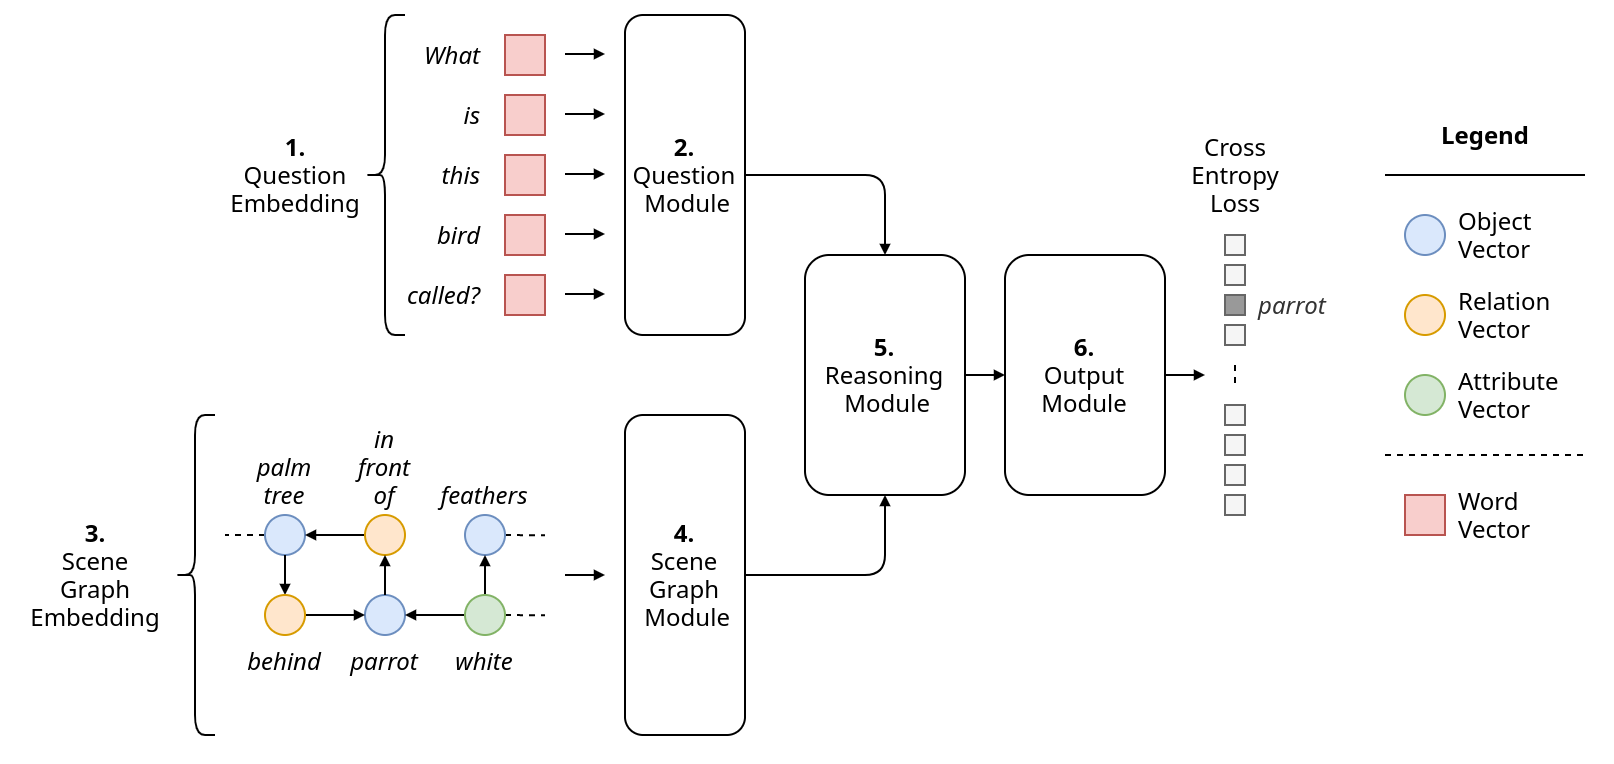
\includegraphics[width=\textwidth]{model_overview.png}
    \caption{A high-level overview of the proposed visual-question-answering model.}
    \label{fig:model_overview}
\end{figure}

The question embedding and question module are responsible for

\section{Question Embedding and Module}
\label{section:question_input_module}

\section{Scene Graph Embedding and Module}
\label{section:scene_graph_input_module}

The primary goal of the scene graph module is to learn a dense representation of scene graph features that can be used as a knowledge-base for the reasoning module to draw information from when answering questions. Both the GQA and CLEVR datasets contain ground-truth scene graph information for each image in the training and validation sets. For GQA, each image is annotated with a global \texttt{location} and \texttt{weather} attribute,  as well as a list of objects, the objects attributes \textit{e.g.} colour, shape, texture and its relations to other objects in the image.

\section{Reasoning Module}
\label{section:reasoning_module}

Given the goal of the question module is to learn a dense contextual and syntactic representation of the question, and the goal of the scene graph module is to capture dependency information between objects, attributes and relations in the scene, we still need to combine and reason about this extracted information. All VQA models have to handle this multi-modal fusion and reasoning in some capacity, with adopting taking fusion-only approaches, whilst others learn self-attention or bidirectional attention weights between question and image modalities, and others leverage the strengths of both methods. For my model, I leverage the reasoning capabilities of the Compositional Attention Network \citeauthor{hudson2018compositional}, a recurrent model that decomposes complex question-answering problems into discrete reasoning steps, each of which is performed by a single cell in the network. The Compositional Attention Network achieved state-of-the-art results on the CLEVR dataset in \citeyear{hudson2018compositional}, achieving 

In order to leverage the computational benefits of sparse tensor operations implemented in PyG \cite{fey2019fast}, I used a PyTorch \cite{paszke2019pytorch} re-implementation of the MAC network, which has been trained to 98.6\% on the CLEVR dataset \cite{eyzaguirre2020differentiable}, just 0.3\% shy of the official result reported by 
\citeauthor{hudson2018compositional}. Notably, this re-implementation accounts for minor details that were omitted from the original MAC network paper but enabled by default in the official MAC network repository {\color{red} citation required}.



\section{Output Module}
\label{section:output_module}

\begin{figure}[htbp]
    \centering
    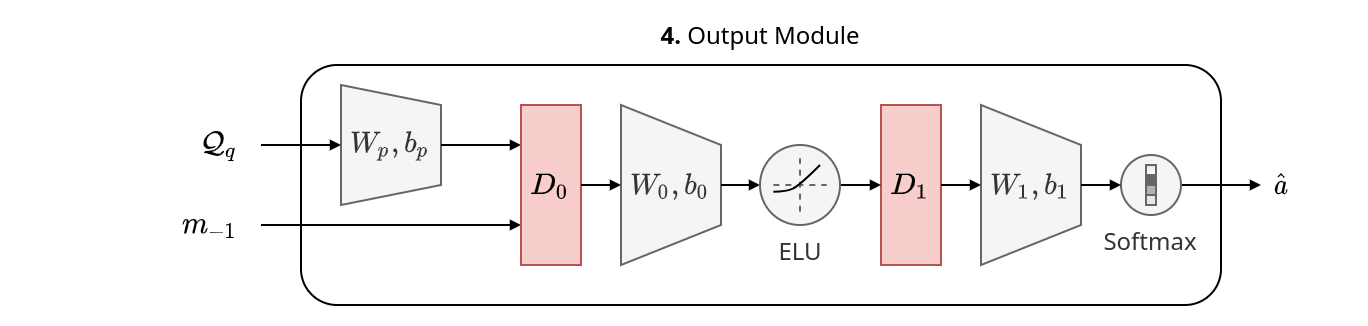
\includegraphics[width=\textwidth]{output_module.png}
    \caption{An overview of the output module, as implemented in the original P}
    \label{fig:output_module}
\end{figure}

{\color{red}

Move to Ablations

\begin{itemize}
  \item Concat + linear fusion (other fusion types?)
  \item Bottom-up
  \item MAC network
\end{itemize}

\subsection{Bottom-up}
\label{subsection:bottom_up}
 ReLU proved to yield higher results over gated tanh when paired with GAT/GCN embeddings. In the original paper, CNN/R-CNN features are extracted in the preprocessing step, meaning there is no need for gradient propagation to the knowledge base embedding. Preliminary tests showed a need for learnable embeddings in graph convolutional models, and thus a need for end-to-end propagation of gradients.}



\begin{itemize}
  \item Initial tests showed little performance difference between conditioning the current control state on previous control states. % #TODOInvestigate interpretability effects
\end{itemize}
